\section{Durchführung}
\label{sec:Durchführung}
\subsection{Aufbau}
Der Versuch wird wie in Abbildung \ref{fig:Aufbau} aufgebaut.
Dabei erfüllen die Rührmotoren den Zweck, die thermisch isolierten Wasserbehälter thermisch homogen zu halten, um eine zuverlässige Temperaturabgabe zu gewährleisten. 
In den Rohren befindet sich ein Gas, welches die Wärme als Phasenumwandlungsenergie transportiert.
Diese wird also wieder abgegeben, wenn das Gas kondensiert, was in Reservoir 1 passiert. 
Danach strömt das Transportmedium als Flüssigkeit bei $T_1$ und $p_{\symup{b}}$ weiter und durch das Drosselventil.
Bei $T_2$ und $p_{\symup{1}}$ verdampft das Transportmedium wieder und wird daraufhin durch den Kompressor komprimiert.
Durch den Druckanstieg kondensiert das Gas wieder und gibt Wärmeenergie an das Wasser in Reservoir 1 ab.
Vor dem Drosselventil befindet sich noch ein Reiniger, der die Flüssigkeit von Gasblasen reinigt.



\begin{figure}[H]
    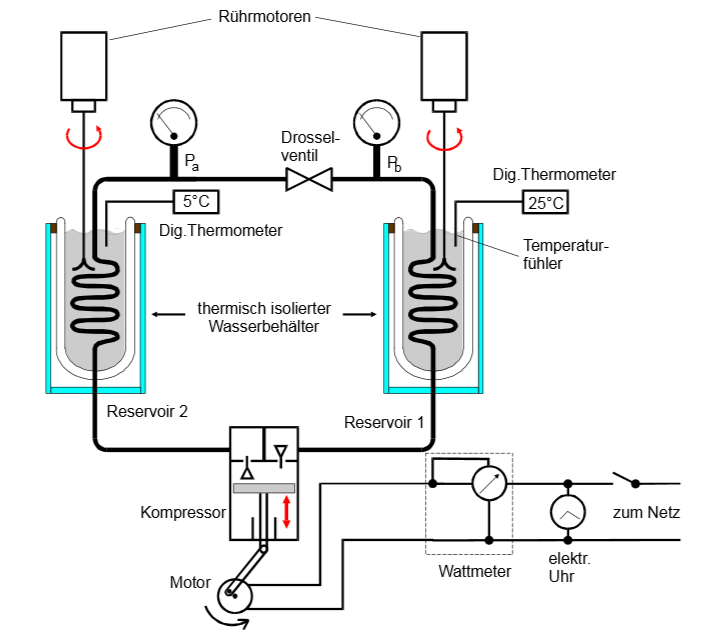
\includegraphics[width=\textwidth]{Bilder/aufbau.png}
    \caption{Abgebildet ist der schematische Aufbau der Wärmepumpe. \cite{V206}}
    \label{fig:Aufbau}
\end{figure}

\subsection{Durchführung}
Die Wasserbehälter werden jeweils mit drei Litern Wasser aufgefüllt und in die Apparatur hinzugefüt.
Der Kompressor wird eingeschaltet, um dann in Abständen von einer Minute die Werte abzulesen.
Diese werden zyklisch in der Reihenfolge $t$, $N$, $p_{\symup{b}}$, $T_1$, $T_2$, $p_{\symup{a}}$ abgelesen, sodass die Zeitdifferenz bei jedem Wert ungeähr gleich ist.
Dadurch kann das Ablesen als gleichzeitig angenommen werden. 
Dies wurde bis zu einer Temperatur von $T_2=0°C$, beziehungsweise $T_1=50°C$ gemacht.